\documentclass[a4paper]{article}

\usepackage[backend=biber, sorting=none]{biblatex}
\usepackage[]{geometry}
\usepackage[font={normalsize,it}]{caption}
\usepackage{titlesec}
\usepackage{graphicx}
\usepackage{subfig}
\usepackage{amsmath}
\usepackage[toc,page]{appendix}
\usepackage{pgfplots}
\usepackage{tikz}
\usepackage{gensymb}
\usepackage[hidelinks]{hyperref}
\usepackage{relsize}
\usepackage{svg}
\usepackage{filecontents}
\usepackage[nottoc,numbib]{tocbibind}
\usepackage{longtable}

\usepackage{mathtools}
\DeclarePairedDelimiter\ceil{\lceil}{\rceil}
\DeclarePairedDelimiter\floor{\lfloor}{\rfloor}

\addbibresource{references.bib}

\renewcommand{\thesection}{\arabic{section}}
\renewcommand{\thesubsection}{\arabic{subsection}}
\renewcommand{\thesubsubsection}{\arabic{subsubsection}}

\titleformat{\section}{\LARGE\sc}{\thesection}{1em}{}
\titleformat{\subsection}{\normalsize\it}{\thesection.\thesubsection}{0.9em}{}
\titleformat{\subsubsection}{\small\it}{\thesection.\thesubsection.\thesubsubsection}{0.9em}{}



\pgfplotsset{compat=1.11,
	/pgfplots/ybar legend/.style={
		/pgfplots/legend image code/.code={%
			\draw[##1,/tikz/.cd,yshift=-0.25em]
			(0cm,0cm) rectangle (3pt,0.8em);},
	},
}
\begin{document}

\begin{titlepage}
\begin{center}

\vspace{1.7cm}

\begin{Huge}
Slum Detection using Multiclass Land Cover in Bangalore
\end{Huge}


\vspace{1.5cm}

Derk Barten\\
11043075

\vspace{1.5cm}

Honors Bachelor thesis extention\\
Credits: 6 EC

\vspace{0.5cm}

Bachelor Opleiding Kunstmatige Intelligentie

\vspace{0.25cm}

University of Amsterdam\\
Faculty of Science\\
Science Park 904\\
1098 XH Amsterdam

\vspace{4cm}

\emph{Supervisor}\\
Dr. Debraj Roy

\vspace{0.25cm}

Department of Computational Science\\
Faculty of Science\\
University of Amsterdam\\
Science Park 904\\
1098 XH  Amsterdam

\vspace{1.5cm}

\today

\end{center}


\end{titlepage}
\thispagestyle{empty}
\clearpage

\section{Introduction}

Informal housing is a common issue faced by cities in developing countries. Inhabitants of informal regions, commonly named as slums, have less social economic opportunities and a lower quality of life compared to urban residents in formal housing. The monitoring of these the development of slums requires resources which governments in developing countries often cannot spare. Remote sensing methods from satellites provide a relatively low cost solution in tracking development of slums in the city. The detection of informal areas from the images provides by satellites remains a difficult task despite the effort from the field of study. This is in part caused by the disparate nature of slums, which varies between cities and even between regions of the same city. The slum characteristics of this type of slum are small buildings which are similar to tents, covered with plastic fabric roofs often colored blue. This type of slum indicates a newly developing slum, which has often a lack of basic services, such as infrastructure and sanitation. Over time, the inhabitants of these slums improve the build quality of the slums into permanent housing. Slum upgrading efforts of the government aim to support these slums by providing the lacking basic services to these newly developed neighborhoods. In this thesis, we focus explicitly on this type of developing slum. The automatic detection of developing slums from satellite images enables the government to support the needs of these developing neighborhoods.

\subsection{Global Context}
% state
According Un-Habitat, close to a third of the global urban population lives in informal settlements \cite{2016state}. In specific parts of the world, for instance Sub-Saharan Africa, the urban population that lives in informal housing is estimated to be close to two thirds of the total urban population \cite{un2013planning}. In the past decades, the percentage of slum inhabitants compared to the urban population has decreased. Paradoxically, in absolute terms, the total number has actually increased \cite{2016state}.

% definition and negative effects
Informal settlements exist globally, although often in different forms and described using different names. The individuals living in informal settlements, such as slum dwellers, are specified by Un-Habitat by one ore more of the following conditions: inadequate  drinking  water,  inadequate  sanitation, poor  structural quality of housing, over crowding and insecurity of tenure \cite{un2015slum}. In addition, the inhabitants of slums experience social and economical exclusion from the opportunities that an urban environment offers. Furthermore, slum dwellers are prone to natural disasters in addition to disease outbreaks. 

% solution
Over the years, there have been multiple governmental policies implemented to address the problem of informal settlements. Informal settlements were largely tolerated and neglected, large eviction and resettlement of the inhabitants were not found to be effective \cite{kuffer2016slums}. Instead, in recent years, a less intrusive approach is used in solving the slum problem. This method enables governments to solve the slum question by supporting the upgrade of slums to formal housing \cite{cobbett2013cities}. Besides government policy, Un-Habitat allocates a significant effort to the use of this method itself\cite{2015globact}.

\subsection{Related works and contributions}
% into remote sensing
In many cities in the developing world, slums are a large part of the urban environment. However, there is often a lack of information about the properties of the slum, such as the location, the scale and the population \cite{kuffer2016slums}. These cities often do not have the resources to obtain this information. Remote sensing is able to provide the often lacking  social economic information. Besides, remote sensing is also able to capture the spatial and temporal dynamics of the informal areas, which supports urban planning and the development of the city.

% methods
In the last decade, access to satellite images was becoming widespread along side an increase in methods for urban area classification \cite{kuffer2016slums}. This allowed for informal areas to be studied throughout the globe, e.g. Colombo \cite{colombo}, Johannesburg \cite{williams2016automatic}, Accra \cite{accra}, Mumbai \cite{mumbai}, Rio de Janeiro \cite{hofmann2008detecting}, and Hyderabad \cite{hyderabad}. With the increase interest in slum detection, it became apparent that the structural characteristics of slums were quite different from formal areas. This led to a large number of approaches based on the extraction of  image based features from satellite images. These approaches are, among others: the presence of vegetation \cite{niebergall2007object}, the size and shapes of buildings \cite{hofmann2008detecting}, the roofing material \cite{williams2016automatic}, texture features \cite{mattia2007exploiting}, and road accesability \cite{owen2013approach}.

Currently, the majority of studies uses the pixel image data of informal regions to extract features \cite{kuffer2016slums}. A different approach would be the characterization of areas by the objects that inhabit them. This is, for example, the detection of individual roofs in a certain area  of an image \cite{williams2016automatic}. Another example of this object based approach is the detection of road systems to characterize image regions. Alternatively, studies have used land use information \cite{novack2010urban} or social economical statistics \cite{engstrom2011using} to detect informal settlements.

% results
% The performance of the methods used in the studies is very variable. There are studies that have achieved a very high accuracy of in the 90\%. 

% conclusion prev work
%Because slums vary incredibly between different cities and regions, it is hard to obtain consensus about characteristics that well define informal areas. This variety makes it hard to create a method that will capture all the types of informal areas. As a result, the results obtained by the studies are quite specific to the studied city or area. 

 
\subsection{Proposed Method}

Our thesis continues with the work performed by Graesser \textit{et al.} \cite{graesser2012image}. The paper characterized formal and informal neighborhoods using a set of different features extracted from satellite images. Their approach was able to successfully characterize the two types of neighborhoods with high accuracy on certain parts of the urban landscape. We will evaluate two of the feature extraction methods described in the paper from Graesser \textit{et al.} and attempt to reproduce similar results with satellite images from Bangalore. These methods are the Histogram of Oriented Gradients and Line support regions. Beyond the replication and evaluation of previous research, the methods of feature extraction used by Graesser \textit{et al.} will be extended with an additional new method. This method creates a feature based on the density of road intersections in an image. The feature created from this method will be compared to the existing features and measured for its performance. The features produced by the three methods will combined and used by a set of different classification methods.
We will evaluate the different classification methods to discover the most suitable classification method for our image and its features. 



\subsection{Data and Area of Study}
The image data used for the thesis is displayed in Figure \ref{fig:sections}d, a larger version of the image is included in appendix A. The content of this image contain a large area of Bangalore, which is the capital city of the Indian state of Karnataka, located in south central India. The city experienced a fast growth population from 8.4 million in 2011 to 12.3 million in 2017, becoming the third largest city in India\cite{popcount2017}. One of the reasons for its sudden growth is the large IT sector together with better living standards and infrastructure. This rapid increase in population has led to a shortage of housing which, in turn, caused an increase in the number slums in the city. At present, the city is estimated to have over two thousand slums. These slums account for 25 to 35 percent of the urban population \cite{roy2018survey}.

The image in Figure \ref{fig:sections}d has a resolution of 52,322 by 31,789 pixels with a filesize of 6.19GiB and extends in latitude and longitude from  (12°54'22.729", 77°31'58.631") in the south west to (12°59'37.414", 77°40'37.776") in the north east. The image was created in 2012 by the earth observation satellite WorldView3 owned by DigitalGlobe. The WorldView3 satellite produces multiple types of images with varying degrees of resolution. The panchromatic images have a resolution of 0.31 meter in contrast to  the multiband images have a significantly lower resolution of 1.24 meter. The project uses pan-sharpened images, which combines the high resolution panchromatic- and the low resolution multiband images to create high resolution RGB images.

% Source of shape files
Besides image data, we also use vector files with the location and shape of the developing slums we aim to detect. These vector files are overlayed in the images in Figure \ref{fig:sections} and mark the location of the slums. The images a to c show that these slums are relatively small in scale compared to the surrounding neighborhoods. These sections show the the dispersed small blue roofs that characterize this type of informal settlement. 

\subsection{Challenges}

The distinction between formal and informal regions is often quite challenging. In some cases, it is hard to differentiate where to draw the border between formal and informal. In this case, formal areas could be visually similar to informal area despite being of a different class. Furthermore, some areas could be annotated incorrectly. All in all, this produces noise in the dataset which presents a problem for correct binary classification of the two classes of regions.

Another challenge encountered in this field is the scarcity of informal settlements.  Even though a large part of the inhabitants of Banglore reside in informal settlements, the type slums we aim to detect are small and highly distributed thoughout the city. Figure \ref{fig:sections}d illustrates this point quite well. A larger view of the distribution of informal settlements in this area is provided in the appendix. The relative small number of slums causes the dataset of formal and informal regions to become quite skewed.

In our case, everything that is not the specific type of slum we are looking for is automatically considered formal. This is actually not in accord with reality since the formal class includes a large range of different types of buildings. Furthermore, fields and lakes in the image are also included in the formal class. Therefore, the formal class should actually be considered as the class that include all things except a specific type of slum. Consequently, the formal regions have a large amount of variance of visual properties in the image. The diverse content of the formal class of visual characteristics might hinder the effectiveness of classification between formal and informal regions. However, this class division is necessary since we do possess the location and shapes of all other neighborhood types.

The large satellite image displayed in Figure \ref{fig:sections}d is transformed into the three smaller sections displayed in Figure \ref{fig:sections} a to c in order to reduce the skewness between the two classes. These sections were selected on the relative prevalence of informal settlements in that specific part of the image. The location of these sections together relative to the complete image are displayed in Figure \ref{fig:sections}d as red squares. The use of these sections should provide a less one-sided class balance and consequently increase classification performance. 


%\begin{figure}
%\centering
%  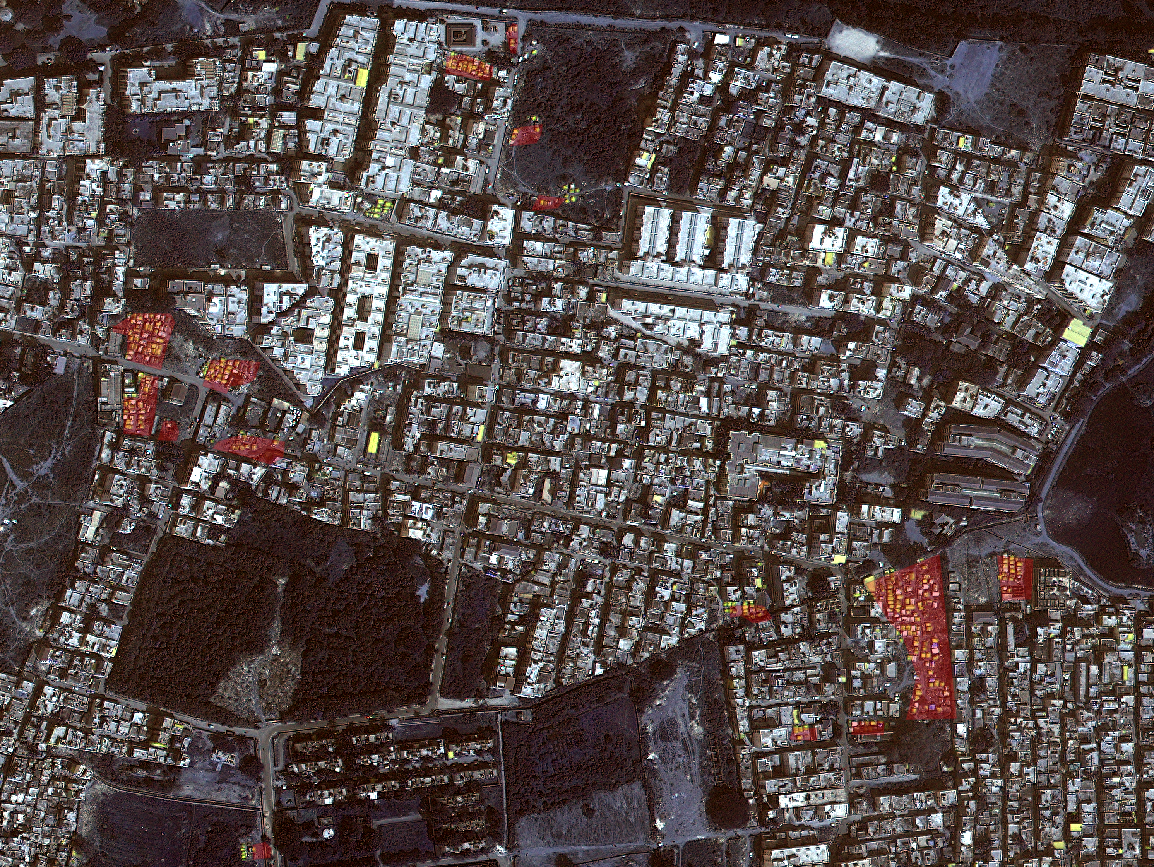
\includegraphics[width=\linewidth]{images/section_3}
%  \caption{Dense informal area in Bangalore, the red patches indicate informal
%  settlements}
%  \label{fig:section_3}
%\end{figure}

\begin{figure}
\centering
\begin{tabular}{cc}
  \subfloat[Section 1]{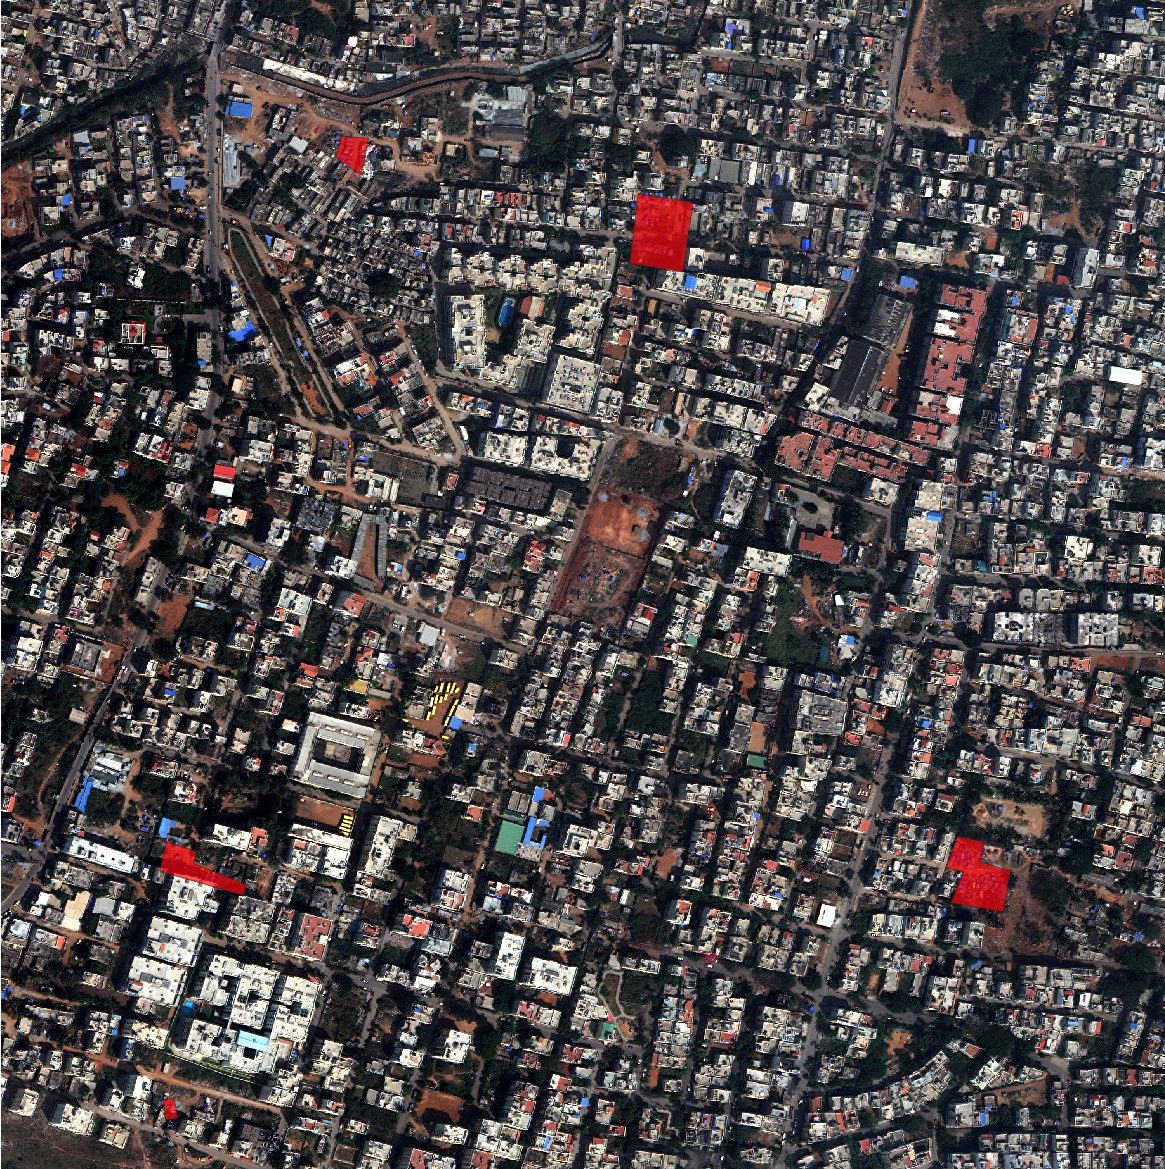
\includegraphics[width=6.2cm, height=5cm]{images/section_1_gt}}&
  \subfloat[Section 2]{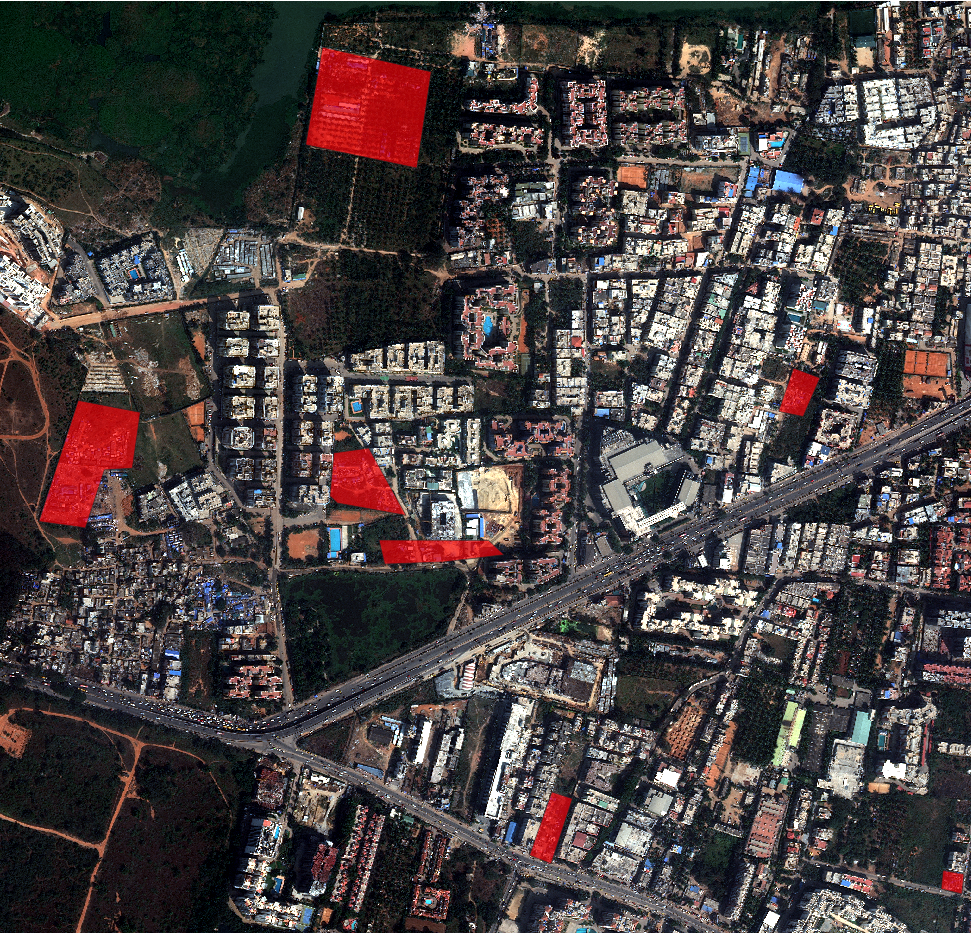
\includegraphics[width=6.2cm, height=5cm]{images/section_2_gt}}\\
  \subfloat[Section 3]{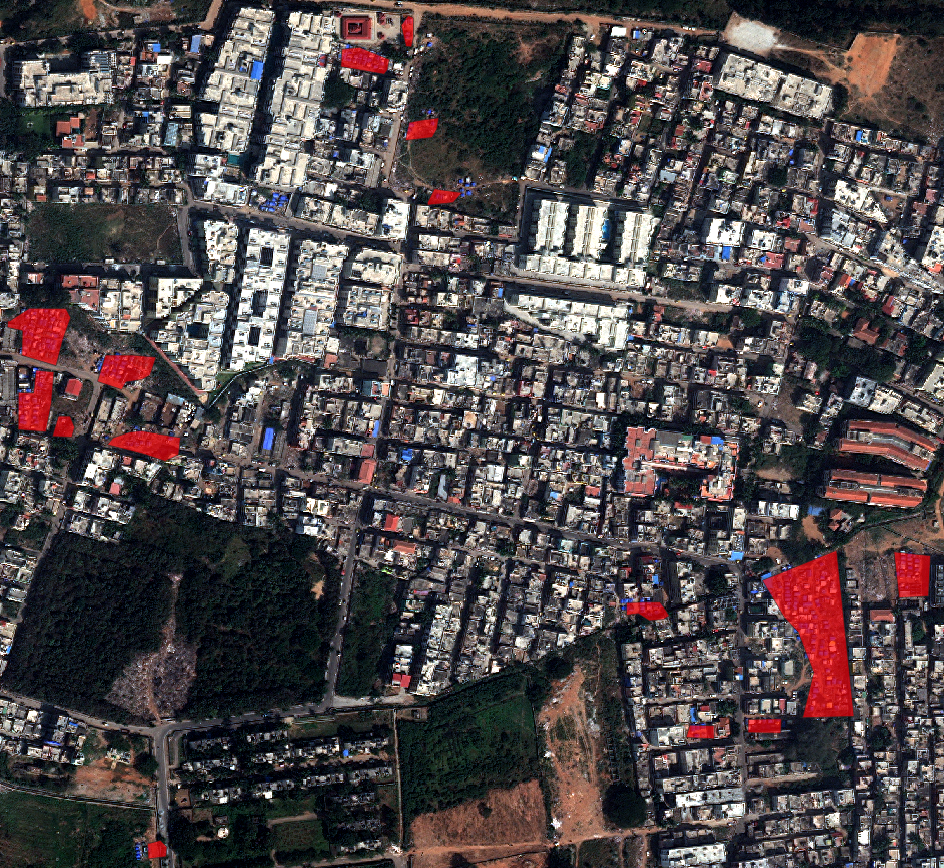
\includegraphics[width=6.2cm, height=5cm]{images/section_3_gt}}&
  \subfloat[Location of Sections]{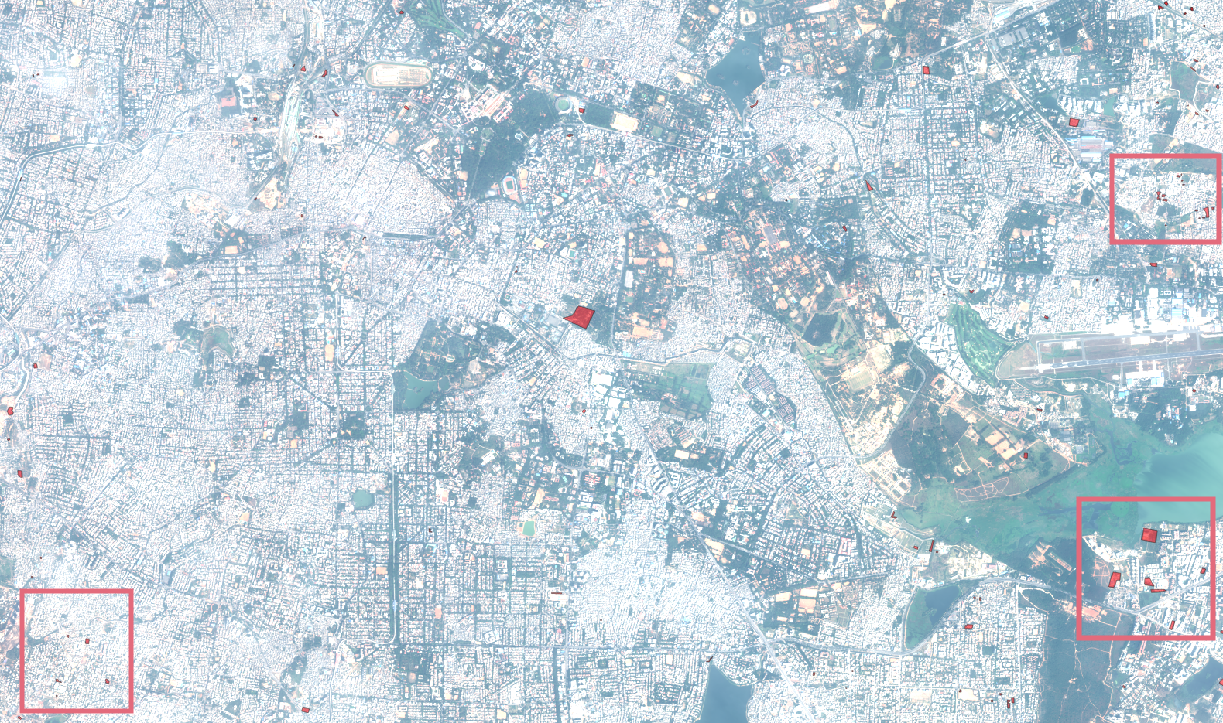
\includegraphics[width=6.2cm]{images/west-bangalore_sections}}
\end{tabular}
\caption{The images used for evaluation and classification}
\label{fig:sections}
\end{figure}



\section{Method}


\subsection{Data}

The image data used are captured by the earth observation satellite WorldView3
owned by DigitalGlobe. The WorldView3 satellite produces multiple categories of
imagery with varying degrees of resolution. The panchromatic images have
a resolution of 0.31 meter in contrast to  the multiband images have
a significantly lower resolution of
1.24 meter. The project uses pansharpened images, which combines the high
resolution panchromatic- and the low resolution multiband images to create
high resolution RGB images.

The content of the images contain regions of Bangalore, which is the capital
city of the indian state of Karnataka, located in south central India. The
population of the city is over ten million and is recognized as a mega city.
Banglore is known to have problems concerning informal settlements. According
to a report from 2012, there are 862 reported slums in the city


\begin{figure*}
  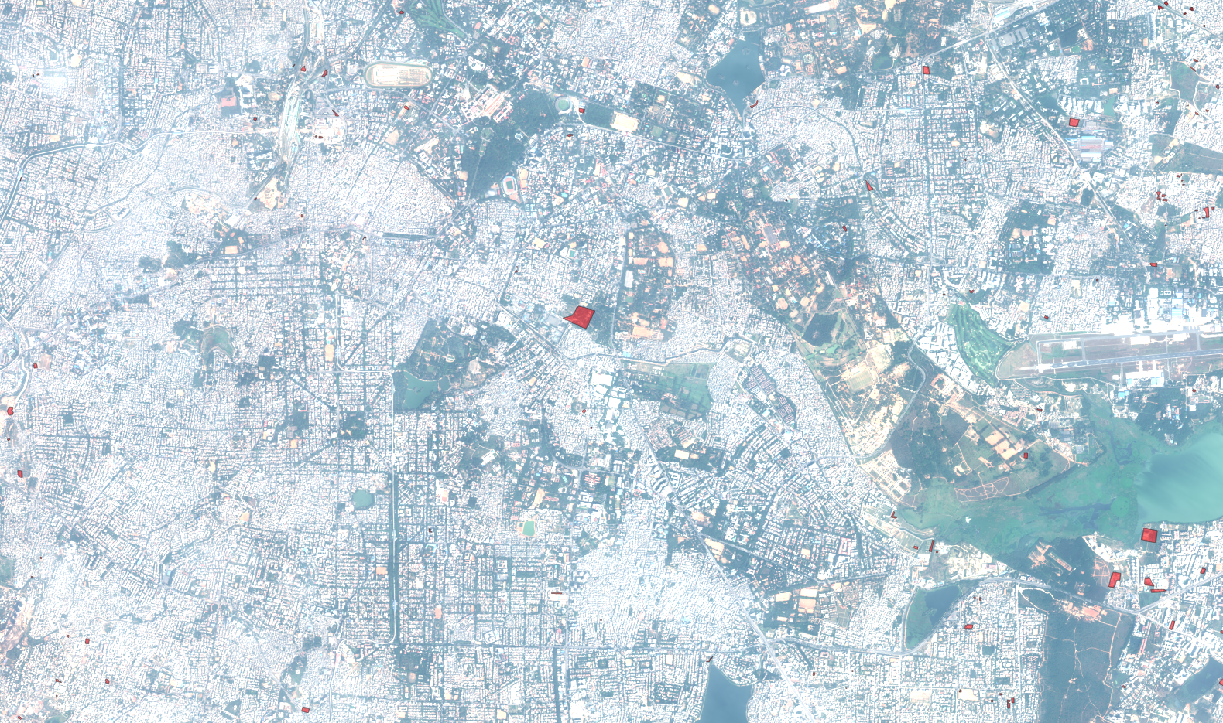
\includegraphics[width=\linewidth]{images/west-bangalore}
  \caption{A part of western Bangalore, the red patches indicate informal
  settlements}
  \label{fig:west-bangalore}
\end{figure*}

\subsection{Challenges}
The distinction between formal and informal regions is often quite challenging,
in part due to the vagueness of borders between the regions. The border between
formal and informal regions often resembles more of a spectrum than a clear cut line.
Besides border difficulties, some areas are not designated as informal, while
still posessing characteristics of an informal region. This results in
a dataset with noise and inconsistency.  All in all, the binary classification
of a region encounters difficulties when applied in practice. 


Another challenge encountered in this field is the scarcity of informal
settlements.  Eventhough Banglore  has an abundance of informal settlements,
the fast majority of land is identified as formal area's. Figure
\ref{fig:west-bangalore} shows a part of western Bangalore where it is clear
that informal settlements are sparce and distributed throughout the city. As
a result, the dataset of formal and informal regions becomes quite skewed.
Furthermore, because everything that is not informal is automatically
considered formal, the formal regions have a large amount of variance of visual
properties.  To illustrate: lakes, forrests, and fields fall in the same
catagory as formal residential and industrial areas while the visual
characteristics are significantly different. The diverse content of the formal
set of visual characteristics might hinder the effectiveness of differentiating
between formal and informal regions. 

To reduce the skewedness between informal and formal, only subsections of Figure \ref{fig:west-bangalore} are
used where the proportion formal to informal is less one-sided. An example of
such a region is Figure \ref{fig:section_3}. A smaller difference in formal
informal ratio allows for a better understanding of the effectiveness of
various features. The features are assesed using these area's 

\begin{figure}
\centering
  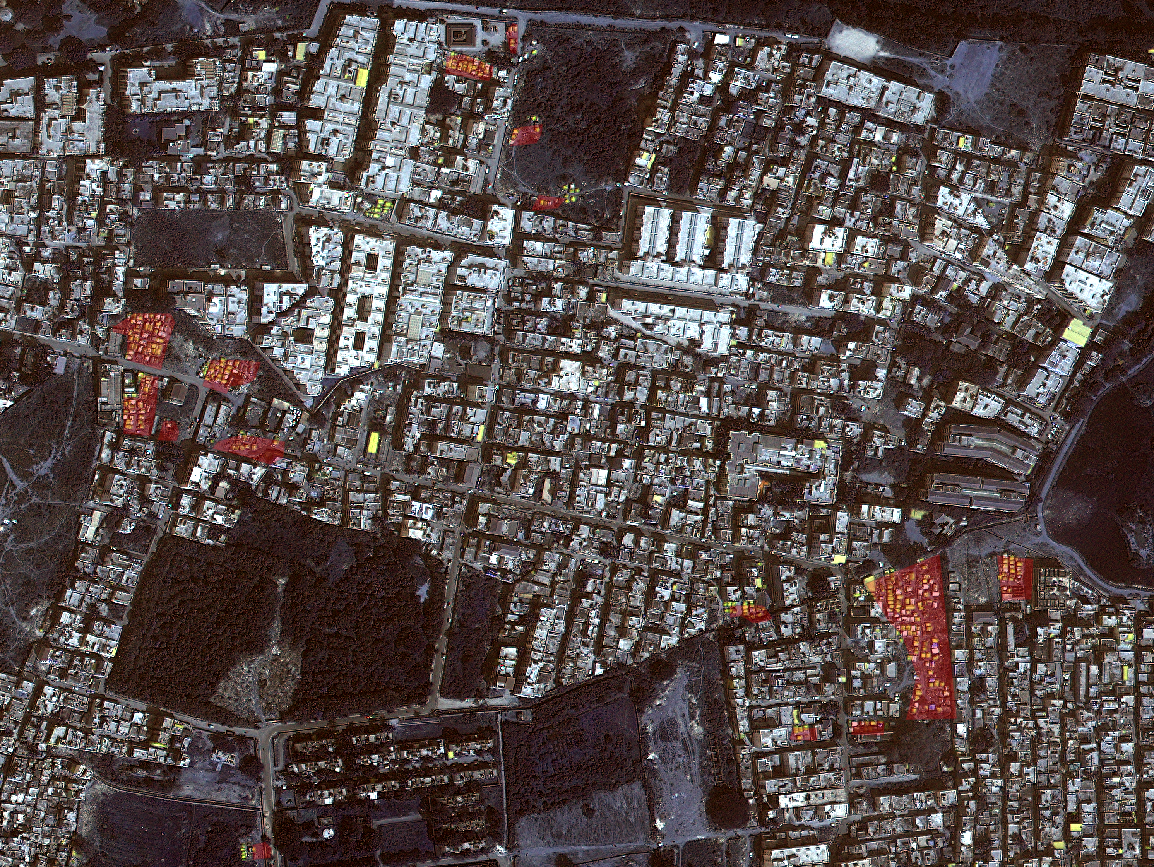
\includegraphics[width=\linewidth]{images/section_3}
  \caption{Dense informal area in Bangalore, the red patches indicate informal
  settlements}
  \label{fig:section_3}
\end{figure}

\subsection{Feature Evaluation}
An important part is the evaluation of the value of estimation that a certain
feature posesses. This allows to conclude if a certain feature is useful in the
discrimination between formal and informal. The use of a set of features allows
for a more solid estimation compared to a single feature by itself. 

The measure of predictive value of a feature is visualized using a boxplot and
the spatial distribution of values. A boxplot for a certain feature, consists
of two classes: the formal and informal class. To latter belong chunks of
pixels that are situated inside formal settlements. The former contains chuncks
that are not within informal regions. In the case that a feature is
distinctive, the distribution of the values in the two classes will be
different. The boxplot visualizes the difference in distribution well, showing
the usefulness of a feature.


\clearpage
\section{Results}

Figure \ref{fig:comp} presents the performance comparison between the two and three class classification using the parameters listed in Table \ref{tbl:params}. This figure shows three metrics for performance: the Mathews Correlation Coefficient (MCC), the F1 score, Precision, and Recall. Both the MCC and the F1 score provide a score that depends on the balance between the precision and recall as these measures alone tend to give wrong impressions of the actual performance. Judging by the MCC and F1 score, for every section, the performance is doubled when using three classes instead of two. Furthermore, there is a significant difference in recall between two class and three class classification.


\pgfplotstableread[col sep = comma]{results/2_vs_3_mcc.csv}\datazero
\pgfplotstableread[col sep = comma]{results/2_vs_3_pre.csv}\dataone
\pgfplotstableread[col sep = comma]{results/2_vs_3_rec.csv}\datatwo
\pgfplotstableread[col sep = comma]{results/2_vs_3_f1.csv}\datafone


\begin{figure}[]
    \begin{tikzpicture}
        \begin{axis}[
            ybar,
            ymajorgrids = true,
            bar width=0.5cm,
            ylabel = Matthews Coefficient,
            width=.5\textwidth,
            height=.5\textwidth,
            enlarge x limits=0.25,
            symbolic x coords={Section 1, Section 2, Section 3},
            xtick=data,
            ymax = 1,
            yticklabel style={
                /pgf/number format/fixed,
                /pgf/number format/precision=2,
                /pgf/number format/fixed zerofill
            },
            scaled y ticks=false,
            ]
            \addplot table[x=TestImage, y=Two]{\datazero};
            \addplot table[x=TestImage, y=Three]{\datazero};
            %\addplot[dotted, sharp plot, update limits=false] coordinates {(0, 0)(1, 0)}; 
            \legend{Two Classes, Three Classes}
        \end{axis}
    \end{tikzpicture}
    \begin{tikzpicture}
        \begin{axis}[
            ybar,
            ymajorgrids = true,
            bar width=0.5cm,
            ylabel = F1 score,
            width=.5\textwidth,
            height=.5\textwidth,
            enlarge x limits=0.25,
            symbolic x coords={Section 1, Section 2, Section 3},
            xtick=data,
            ymax = 1,
            yticklabel style={
                /pgf/number format/fixed,
                /pgf/number format/precision=2,
                /pgf/number format/fixed zerofill
            },
            scaled y ticks=false,
            ]
            \addplot table[x=TestImage, y=Two]{\datafone};
            \addplot table[x=TestImage, y=Three]{\datafone};
            %\addplot[dotted, sharp plot, update limits=false] coordinates {(0, 0)(1, 0)}; 
            \legend{Two Classes, Three Classes}
        \end{axis}
    \end{tikzpicture}
    \begin{tikzpicture}
        \begin{axis}[
            ybar,
            ymajorgrids = true,
            bar width=0.5cm,
            ylabel = Precision,
            width=.5\textwidth,
            height=.5\textwidth,
            enlarge x limits=0.25,
            symbolic x coords={Section 1, Section 2, Section 3},
            xtick=data,
            ymax = 1,
            yticklabel style={
                /pgf/number format/fixed,
                /pgf/number format/precision=2,
                /pgf/number format/fixed zerofill
            },
            scaled y ticks=false,
            ]
            \addplot table[x=TestImage, y=Two]{\dataone};
            \addplot table[x=TestImage, y=Three]{\dataone};
            %\addplot[dotted, sharp plot, update limits=false] coordinates {(0, 0)(1, 0)}; 
            \legend{Two Classes, Three Classes}
        \end{axis}
    \end{tikzpicture}
    \begin{tikzpicture}
        \begin{axis}[
            ybar,
            ymajorgrids = true,
            bar width=0.5cm,
            ylabel = Recall,
            width=.5\textwidth,
            height=.5\textwidth,
            enlarge x limits=0.25,
            symbolic x coords={Section 1, Section 2, Section 3},
            xtick=data,
            ymax = 1,
            yticklabel style={
                /pgf/number format/fixed,
                /pgf/number format/precision=2,
                /pgf/number format/fixed zerofill
            },
            scaled y ticks=false,
            ]
            \addplot table[x=TestImage, y=Two]{\datatwo};
            \addplot table[x=TestImage, y=Three]{\datatwo};
            %\addplot[dotted, sharp plot, update limits=false] coordinates {(0, 0)(1, 0)}; 
            \legend{Two Classes, Three Classes}
        \end{axis}
    \end{tikzpicture}
    \caption{Performance comparison between two and three class classification}
    \label{fig:comp}
\end{figure}


We have provided a visualization of the detected slums for the three-class method in Figure \ref{fig:comp}. In the calculation of the performance and the visualization of the predictions,  we collapse the three classes into two classes after classification. This is motivated by the fact that we are not interested in how well the vegetation or buildings are classified, we only care about the performance of the slum classification compared to everything that is not a slum, the three classes are only used during training and classification. We create two classes from three classes by combining all vegetation and building into a single class. This keeps the comparison between two class and three class classification fair. As a result, the images displayed in Figure \ref{fig:three_classes} display only two classes even though it was trained and tested using three classes.

\begin{figure}[ht]
    \centering
    \begin{tabular}{ccc}
        \subfloat[Section 1 Prediction]{\includegraphics[height=0.28\textwidth]{s1}}&
        \subfloat[Section 2 Prediction]{\includegraphics[height=0.28\textwidth]{s2}}&
        \subfloat[Section 3 Prediction]{\includegraphics[height=0.28\textwidth]{s3}}\\
        \subfloat[Section 1 Ground Truth]{\includegraphics[height=0.28\textwidth]{s1_g}}&
        
        \subfloat[Section 2 Ground Truth]{\includegraphics[height=0.28\textwidth]{s2_g}}&
    
        \subfloat[Section 3 Ground Truth]{\includegraphics[height=0.28\textwidth]{s3_g}}\\
    \end{tabular}
    \caption{Comparison of the three sections between the detected slums in the left column and the ground truth right column. The red patches indicate slums.}
    \label{fig:three_classes}
\end{figure}


\pgfplotstableread[col sep = comma]{results/block.csv}\datablock
\pgfplotstableread[col sep = comma]{results/treshold.csv}\datatreshold

\begin{figure}[ht]
    \centering
    \begin{tikzpicture}
    \begin{axis}[
        ymajorgrids = true,
        bar width=0.5cm,
        ylabel = Performance,
        xlabel = Block Size,
        width=.5\textwidth,
        height=.5\textwidth,
        enlarge x limits=0.25,
        symbolic x coords={10, 20, 30},
        xtick=data,
        ymax = 1,
        yticklabel style={
            /pgf/number format/fixed,
            /pgf/number format/precision=2,
            /pgf/number format/fixed zerofill
        },
        scaled y ticks=false,
        legend pos=north west,
        ]
        \addplot table[x=BlockSize, y=MCC]{\datablock};
        \addplot table[x=BlockSize, y=Precision]{\datablock};
        \addplot table[x=BlockSize, y=Recall]{\datablock};
        %\addplot[dotted, sharp plot, update limits=false] coordinates {(0, 0)(1, 0)}; 
        \legend{MCC, Precision, Recall}
        \end{axis}
    \end{tikzpicture}
    \begin{tikzpicture}
    \begin{axis}[
    ymajorgrids = true,
    bar width=0.5cm,
    ylabel = Matthews Coefficient,
    xlabel = Threshold,
    width=.5\textwidth,
    height=.5\textwidth,
    enlarge x limits=0.25,
    symbolic x coords={0.34, 0.5, 0.8},
    xtick=data,
    ymax = 1,
    yticklabel style={
        /pgf/number format/fixed,
        /pgf/number format/precision=2,
        /pgf/number format/fixed zerofill
    },
    scaled y ticks=false,
    legend pos=north west,
    ]
    \addplot table[x=Threshold, y=MCC]{\datatreshold};
    \addplot table[x=Threshold, y=Precision]{\datatreshold};
    \addplot table[x=Threshold, y=Recall]{\datatreshold};
    %\addplot[dotted, sharp plot, update limits=false] coordinates {(0, 0)(1, 0)}; 
    \legend{MCC, Precision, Recall}
    \end{axis}
    \end{tikzpicture}
    \caption{Performance effect of different block size and threshold for section 3}
    \label{fig:block_comp}
\end{figure}

\begin{figure}[ht]
    \centering
    \begin{tabular}{cc}
        \subfloat[Block Size 10]{\includegraphics[height=0.35\textwidth]{s3}}&
        \subfloat[Block Size 20]{\includegraphics[height=0.35\textwidth]{s3_b20}}\\
        \subfloat[Block Size 30]{\includegraphics[height=0.35\textwidth]{s3_b30}}&
        \subfloat[Ground Truth]{\includegraphics[height=0.35\textwidth]{s3_g}}\\
    \end{tabular}
    \caption{Comparision of the visual difference with increased block size for section 3}
    \label{fig:block}
\end{figure}


We further experimented with different block sizes and thresholds to discover the effects on performance. These experiments are displayed in Figure \ref{fig:block_comp}. Block sizes larger than 10 seem to decrease the MCC and precision while increasing the recall. Increasing the threshold seems to be correlated with increased performance.

\clearpage
\pgfplotstableread[col sep = comma]{results/oversampling.csv}\dataoversampling

\begin{figure}[ht]
    \centering
    \begin{tikzpicture}
    \begin{axis}[
    ybar,
    ymajorgrids = true,
    bar width=0.5cm,
    ylabel = Matthews Coefficient,
    xlabel = Amount of Oversampling,
    width=.5\textwidth,
    height=.5\textwidth,
    enlarge x limits=0.25,
    symbolic x coords={x2, x4, Equal},
    xtick=data,
    ymax = 1,
    yticklabel style={
        /pgf/number format/fixed,
        /pgf/number format/precision=2,
        /pgf/number format/fixed zerofill
    },
    scaled y ticks=false,
    legend pos=north west,
    ]
    \addplot table[x=Performance, y=MCC]{\dataoversampling};
    %\addplot[dotted, sharp plot, update limits=false] coordinates {(0, 0)(1, 0)}; 
    \legend{}
    \end{axis}
    \end{tikzpicture}
    \caption{Performance effect of oversampling of the slum class in section 3}
\label{fig:oversampling_comp}
\end{figure}

Figure \ref{fig:oversampling_comp} visualizes the impact of oversampling the slum class. The cases of two times and four times refer to the size of the slum class that was multiplied by two and four respectively. The last column is the case where all classes are oversampled to have the same number of entries.


\clearpage
\section{Discussion}
There is a clear improvement when using three classes instead of two, as displayed in Figure \ref{fig:comp}. Because the MCC and F1 score both use the precision and recall, it is likely that the increase in recall caused the increase of these two measures. With three classes for the third section, it seems that it is able to keep a high recall when the precision is high. In contrast, the two class classification has a significantly lower recall while the precision is equal to that of the three class classification. The improved performance results in relatively accurate predictions with very little noise, with the exception of the first section, as visualized in \ref{fig:three_classes}.

Interestingly enough, Figure \ref{fig:three_classes}c seems to detects traffic as areas of slum. Upon further investigation, the morphology of cars on the road seems to match that of slums. On satellite images, cars resemble small scattered, disorganized, objects, thus both appearance and in texture similar to slums. This effect is perhaps enlarged by the fact that the features that are used are largely based on texture. Furthermore, the other two images that are used for training do not contain large amounts of traffic, therefore the algorithm has not learned that these vehicles are not slums.

The experiment with the different block sizes suggests that performance drops when increasing block size. 





 
%\section{Conclusion}

Our approach was able to detect slums on the provided images, albeit to a certain extend. We have experimented with different sets of parameters to find the best combination, which produced Matthews Coefficient of 0.17. We found that the Histogram of Gradients and GradientBoosting generally achieves the highest performed. Our proposed method for the detection of slums using road detection did not seem to produce useful results, although the intersection detection might be applicable for different problems. The effect of different scales is still debatable however increased block size did not seem to impact performance of the features.



% Summary of results, which parameters worked well
% Reached goal?






%\section{Future Work}
%As you now know, we performed the experiments on three test images. These images are only a small part of the whole image. This was done to reduce computational load and decrease the class imbalance. We have not classified using the whole image, although this could be the next logical step.
%
%would be classification of the whole image as a test set, and the three sections as training set. 


% future work: make 4 classes, or even 5 using soil and water. perhaps more classes leads to diminishing returns eventually

%\addcontentsline{toc}{section}{References}
\clearpage
\printbibliography
\end{document}

